\documentclass[main.tex]{subfiles}
\begin{document}
\section{Visualization \& Insights}
The distributed architecture implemented in this project has been to facilitate the ability to query crime data and have it presented in a readable fashion. This is primarily through use of a heat map which has the advantage of visualizing large amounts of data as patterns based on the output data of the BKM clustering algorithm. It is also possible to perform SQL queries on the data stored in the HDFS through use of Drill hosted on a server with access to the HDFS. The histogram chart shown in figure \ref{fig:crimeMonths} depicts an example of a resulting visualisation from SQL queries to show crime data for each month in 2018. The data has been visualized using Vega Lite \cite{VegaLite}. 

\begin{figure}[H]
    \centering
    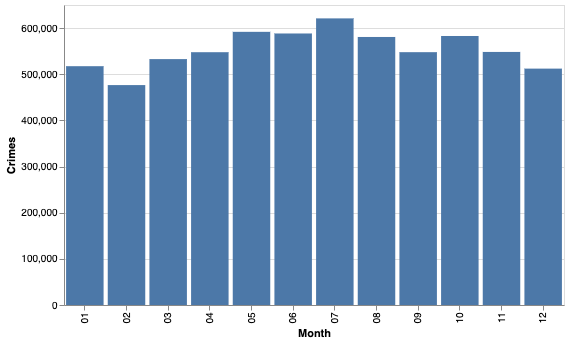
\includegraphics{Images/CrimeMonths.png}
    \caption{Recorded crimes per month in England, Wales and Northern Ireland}
    \label{fig:crimeMonths}
\end{figure}

\subsection{Bisecting K-Means Heat Map}
%Two heat maps are presented in this example to show the effect that the BKM clustering algorithm has on the data points and the information they represent. These heat maps use that same data set over crimes from October 2019. The heat map in figure \todoL{put unclustered heat map and ref} shows crime data points that have not been pre-processed using BKM. The heat map in figure \todoL{put and ref clustered heat map} shows data points that \textit{have} been clustered. %Say some smart shit, less memory, same information, bla bla


This section justifies the use of heat maps as a way of visualizing crime data and then heat maps are used to assess if the bisecting k-means clustering algorithm is able to reduce the amount of observations in the original data while preserving patterns. Reducing the observations has the potential to limit the work load of visualization tools while making the data easier for humans to interpret by reducing noise. Data presented in this section is limited to the 2018 street crimes for the Metropolitan and City of London police forces due to the limited access to computing resources for running bisecting k-means.

Heat maps are able to present high density observations in gradient colors ranging between blue, cyan, green, yellow and red. Each point can be assigned a weight which increases color intensity. The weight property is useful when representing the amount of observations within a given cluster. A regular map of data points is not able to visualize a large amount of unweighted points very well because the map is most likely cluttered with noise. \autoref{fig:2018-01-street-crime-metropolitan-city-of-london} (a) shows 85 004 points which makes the map hard to read and interpret because points are stacked on one another. It is possible to reduce the noise by using a heat map without clustering as shown in \autoref{fig:2018-01-street-crime-metropolitan-city-of-london} (b). But one disadvantage of this approach is that many of the points are stacked. Instead it is more preferable to cluster points that are close together and assign a larger weight to dense clusters. The weight is calculated based on the cluster size by using min-max normalization. \autoref{fig:2018-01-street-crime-metropolitan-city-of-london} (c) shows a heat map where the amount of observations are reduced by approximately 66\% from 85 004 to 28 882. There are visible changes in the color representation but the overall pattern remains intact. Reducing the amount of observations by approximately 83\% from 85 004 to 14 771 still preserves major patterns and clusters are more concentrated as shown in \autoref{fig:2018-01-street-crime-metropolitan-city-of-london} (d). Lastly as seen in \autoref{fig:2018-01-street-crime-metropolitan-city-of-london} (e), by reducing the amount of observations by approximately 94\%, the clusters are beginning to spread to almost the point where some of them begins to separate.

\begin{figure}[H]
    \centering
    \subfloat[85 004 observations]{{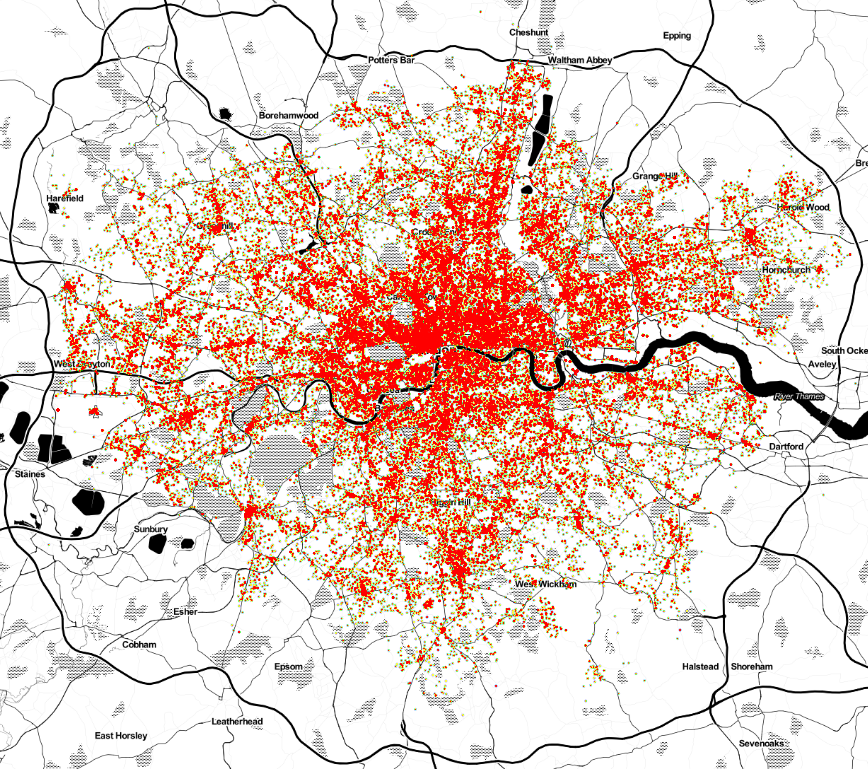
\includegraphics[width=0.45\textwidth]{Images/ml/2018-01-raw-inner-london.png} }}
    \qquad
    \subfloat[85 004 observations heatmap]{{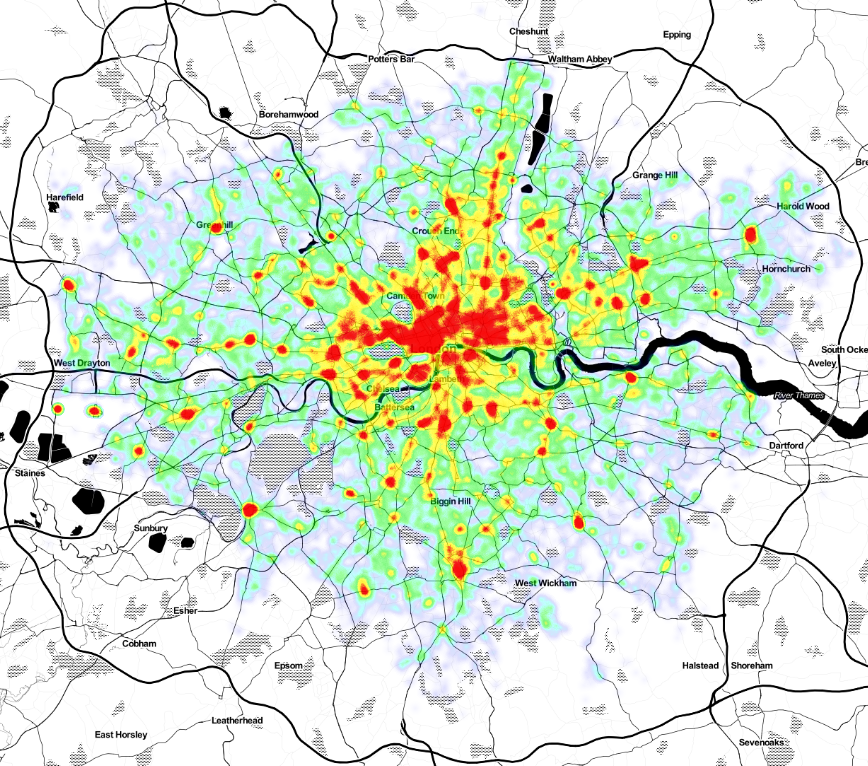
\includegraphics[width=0.45\textwidth]{Images/ml/2018-01-raw-inner-london-heatmap.png} }}
    %\caption{2018-01 Street Crime, Metropolitan \& City of London}
    \subfloat[28 882 clusters heatmap]{{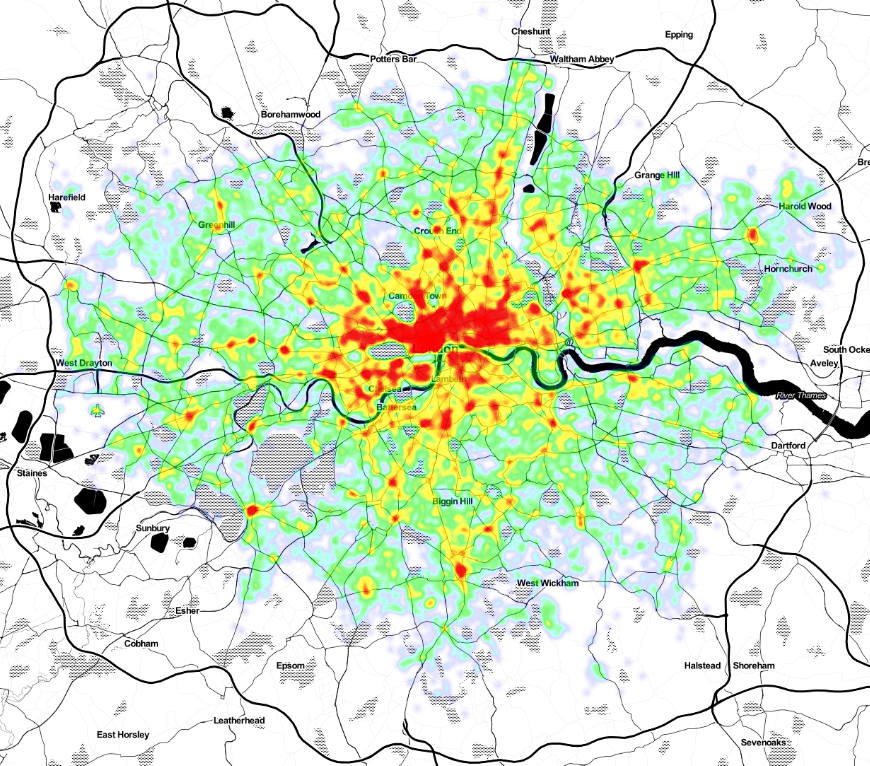
\includegraphics[width=0.45\textwidth]{Images/ml/2018-01-inner-london-k-50000-heatmap.png} }}
    \qquad
    \subfloat[14 771 clusters heatmap]{{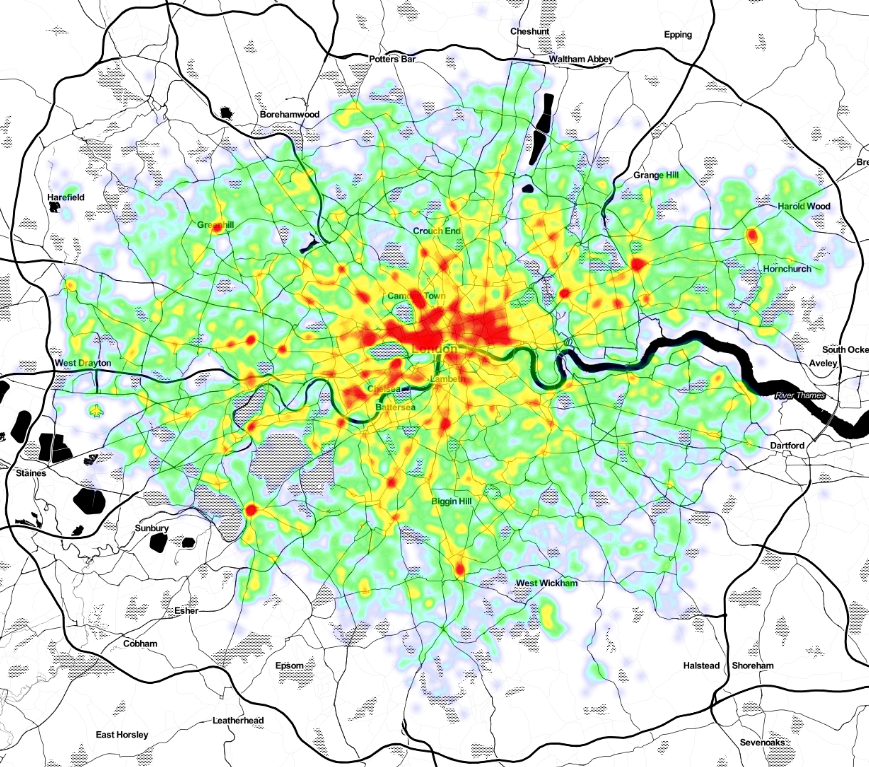
\includegraphics[width=0.45\textwidth]{Images/ml/2018-01-inner-london-k-15000-heatmap.png} }}
    %\caption{2018-01 Clustered Street Crime, Metropolitan \& City of London}
    \subfloat[4 996 clusters heatmap]{{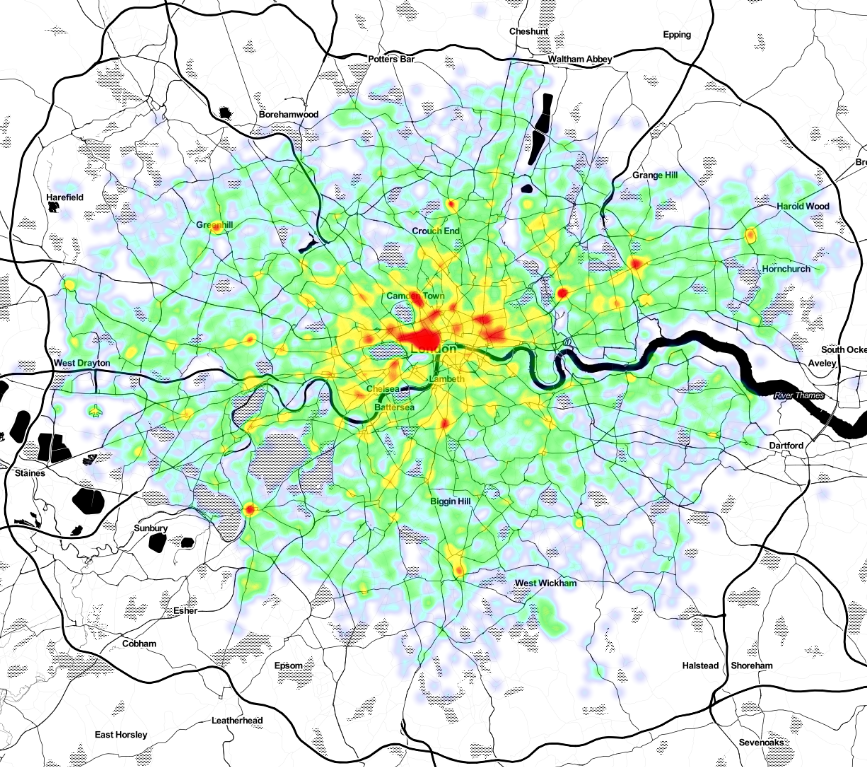
\includegraphics[width=0.45\textwidth]{Images/ml/2018-01-inner-london-k-5000-heatmap.png} }}
    \caption{2018-01 Street Crime, Metropolitan \& City of London Police Forces}
    \label{fig:2018-01-street-crime-metropolitan-city-of-london}
\end{figure}

For this zoom level on the map, analysing between 15 000-30 000 clusters reduces noise while still preserving patterns from the original data. If the zoom level increases the amount of clusters could be increased and likewise if the zoom level decreases, the amount of clusters could be decreased. To illustrate this consider \autoref{fig:2018-01-street-crime-metropolitan-city-of-london-zoom} where a higher amount of clusters provides a more smooth and detailed heat map when the zoom level increases.

\begin{figure}[H]
    \centering
    \subfloat[28 882 clusters heatmap zoom]{{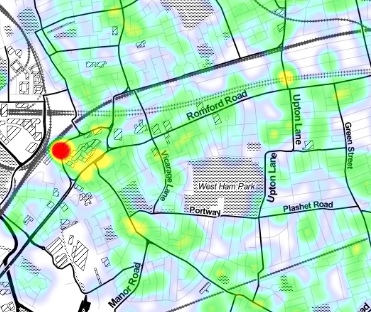
\includegraphics[width=0.45\textwidth]{Images/ml/2018-01-inner-london-k-50000-heatmap-zoom.png} }}
    %\caption{2018-01 Clustered Street Crime, Metropolitan \& City of London}
    \subfloat[4 996 clusters heatmap zoom]{{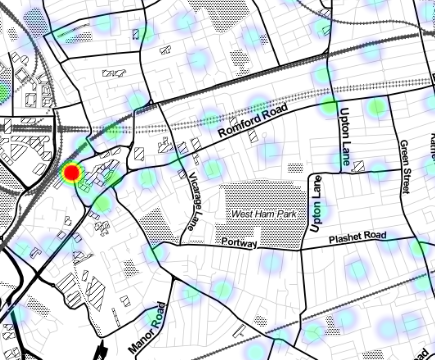
\includegraphics[width=0.45\textwidth]{Images/ml/2018-01-inner-london-k-5000-heatmap-zoom.png} }}
    \caption{2018-01 Street Crime, Metropolitan \& City of London Police Forces Zoom}
    \label{fig:2018-01-street-crime-metropolitan-city-of-london-zoom}
\end{figure}

Another problem that occurs when increasing the zoom level is that the difference in cluster weights becomes too small to notice any difference between cluster sizes. This problem is illustrated on \autoref{fig:2018-01-street-crime-metropolitan-city-of-london-weight-normalization} (a) where the difference in the gradient colors are very subtle to notice a difference. Furthermore, the problem results in the cluster of size 19 is more blue (i.e. lower on the gradient scale) where clusters that blends together but have a lower total is more green (higher on the gradient scale). This problem was solved by adjusting the cluster weights by min-max normalizing only the visible cluster's weights. This ensures that the visible clusters are assigned colors dynamically ranging from the lowest to the highest possible value on the gradient scale as seen in \autoref{fig:2018-01-street-crime-metropolitan-city-of-london-weight-normalization} (b).

\begin{figure}[H]
    \centering
    \subfloat[Normalization across all clusters]{{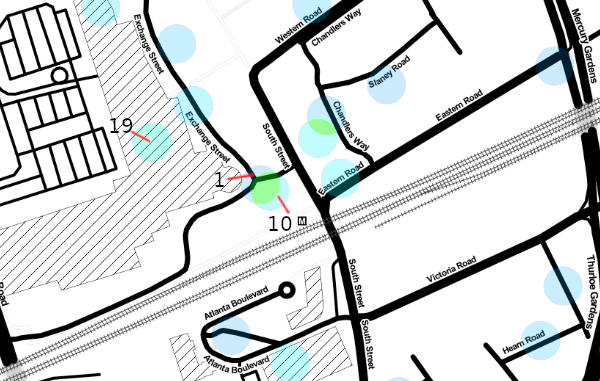
\includegraphics[width=0.45\textwidth]{Images/ml/flaws/cluster-heatmap-flaw.png} }}
    %\caption{2018-01 Clustered Street Crime, Metropolitan \& City of London}
    \subfloat[Normalization across visible clusters ]{{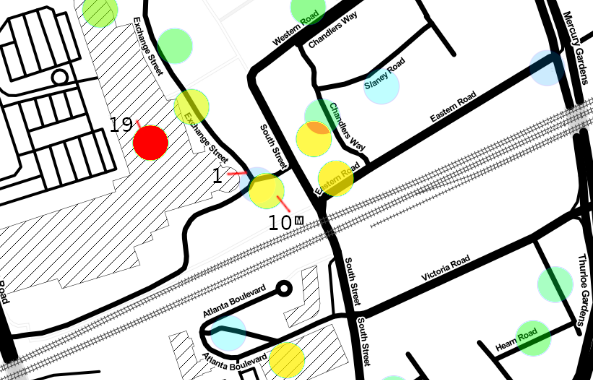
\includegraphics[width=0.45\textwidth]{Images/ml/flaws/cluster-heatmap-flaw-fix.png} }}
    \caption{2018-01 Street Crime, Metropolitan \& City of London Police Forces Weight Normalization}
    \label{fig:2018-01-street-crime-metropolitan-city-of-london-weight-normalization}
\end{figure}

\autoref{fig:2018-01-street-crime-metropolitan-city-of-london-comparison} shows a comparison of the clustered heat map and the UK's Police web query interface for crime data. UK's Police UI makes use of a clustering technique that splits the clusters as the zoom-level increases and merges clusters as zoom-level decreases. Furthermore, only data for an area with boundaries can be investigated. This approach works well for showing numbers but it may be missing some level of detail in the visualization, because clusters change their centroids once they are merged or split. The heat map preserves all clusters including centroids without boundaries by blending instead of merging them together. 

\begin{figure}[H]
    \centering
    \subfloat[Merged Clusters provided by UK Police\cite{dataPolice201801Ramford} ]{{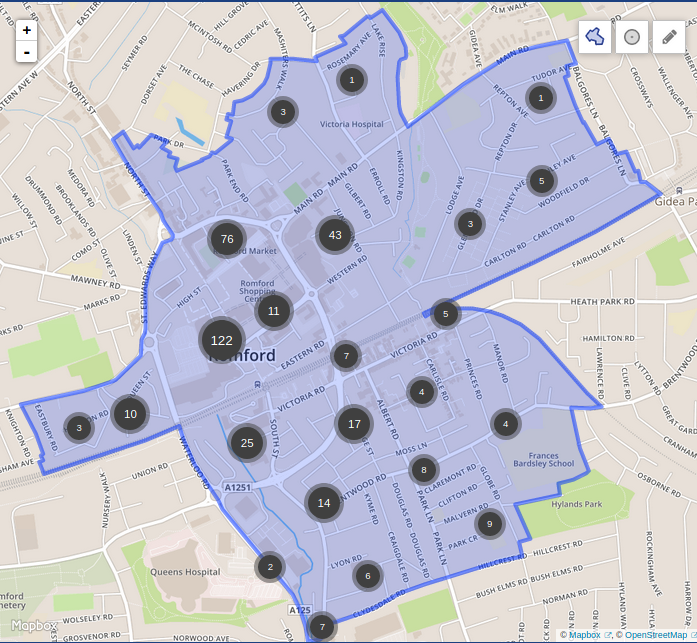
\includegraphics[width=0.45\textwidth]{Images/ml/flaws/2018-01-police-uk-ramford.png} }}
    \subfloat[Heatmap normalized across visible clusters ]{{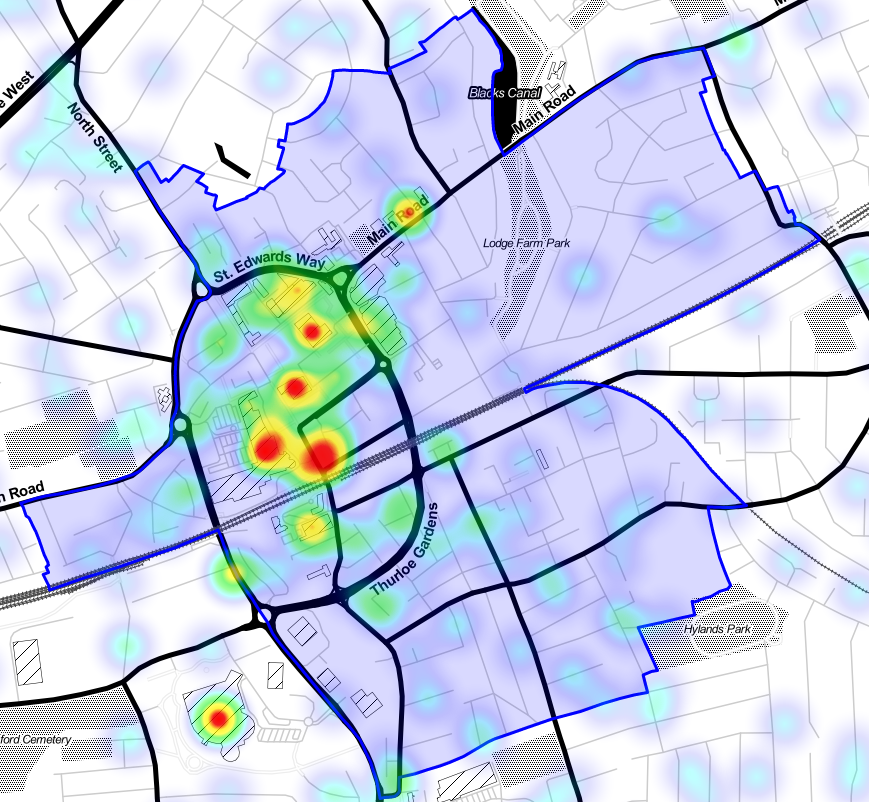
\includegraphics[width=0.45\textwidth]{Images/ml/flaws/2018-01-ramford-heatmap-radius20-blur22.png} }}
    \caption{2018-01 Street Crime, Metropolitan \& City of London Police Forces Comparison of Merging Clusters and Heatmap}
    \label{fig:2018-01-street-crime-metropolitan-city-of-london-comparison}
\end{figure}

\end{document}